\documentclass{article}

% =====================================================================
%  WORKSHOP SWITCH -- uncomment exactly ONE of the two lines below.
%  Everything that differs between the two submissions (title, venue
%  string, abstract, intro, discussion) lives in that file; the rest of
%  this document is shared verbatim.
% =====================================================================
\newcommand{\WKFILE}{workshop-ai4good}
%\newcommand{\WKFILE}{workshop-privacy}
% =====================================================================

% ---------------------------------------------------------------------
%  ANONYMITY SWITCH.  `dblblindworkshop` prints "Anonymous Author(s)"
%  and ignores the \author block below entirely, so the real names can
%  stay in the source at all times.  For a single-blind venue or the
%  camera-ready, swap in `sglblindworkshop` and the block prints.
% ---------------------------------------------------------------------
\usepackage[dblblindworkshop]{neurips_2026}
%\usepackage[sglblindworkshop]{neurips_2026}

\usepackage[utf8]{inputenc}
\usepackage[T1]{fontenc}
\usepackage{hyperref}
\usepackage{url}
\usepackage{booktabs}
\usepackage{amsfonts}
\usepackage{amssymb}
\usepackage{amsmath}
\usepackage{nicefrac}
\usepackage{microtype}
\usepackage[dvipsnames]{xcolor}
\usepackage{graphicx}
\usepackage{soul}

\newcommand{\martine}[1]{\textcolor{magenta}{Martine: #1}}
\newcommand{\s}[1]{\textcolor{Dandelion}{Steven: #1}}

\input{\WKFILE}

\title{\wkTitle}
\workshoptitle{\wkVenue}

\author{%
  Steven Golob\thanks{Corresponding author.} \\
  University of Washington Tacoma \\
  \texttt{golobs@uw.edu} \\
  \And
  Sikha Pentyala \\
  University of Washington Tacoma \\
  \And
  Martine De Cock \\
  University of Washington Tacoma \\
}

\begin{document}

\maketitle

\begin{abstract}
\wkAbstract
\end{abstract}

% =====================================================================
\section{Introduction}
% =====================================================================
\wkIntro

% =====================================================================
\section{Background and related work}
\label{sec:related}
% =====================================================================

\paragraph{DECAF: fairness as graph surgery.}
DECAF \citep{vanbreugel2021decaf} generates fair synthetic tables from a GAN
whose generator is \emph{factored} along a causal DAG (directed acyclic
graph): the joint distribution over columns is written as a product of
conditionals, $P(X) = \prod_i P(X_i \mid \mathrm{pa}(X_i))$, with
$\mathrm{pa}(X_i)$ the columns the graph draws as parents of column $X_i$.
This is similar to the decomposition a marginals-based synthesizer such as
MST fits, differing chiefly in that MST's dependency graph is undirected \martine{Need to cite MST paper already here, with the first mention of MST}.
DECAF gives each column its own sub-network reading only $\mathrm{pa}(X_i)$,
so a parent can be severed at generation time by substituting an independently
drawn surrogate, leaving the generator structurally unable to use the unfair
pathway and \hl{requiring no retraining} \martine{I understood from the rest of the paper that the DAG in DECAF is manually created, so there is no structure learning going on in any case. What about parameter learning, i.e., learning the conditional probability distributions? When you change the graph, don't you need to estimate/measure those new conditional probability distributions? Doesn't that count as training? If not, then what do you consider ``training'' in the DECAF context in the first place (since you talk about ``re-training'')?} \s{I agree that this needs clarifying / revising to be clear. I believe that cuts in DECAF really just ignore those conditional probabilities, and are based on a surrogate (uniformly distributed?) parent, with no conditional attached to it, or the conditional is the same with a uniformly distributed parent? Need to check on this.}.

Which edges to sever turns a fairness \emph{definition} into an
\emph{algorithm}, and DECAF supplies three (Figure~\ref{fig:pruning}).
\textbf{FTU} (fairness through unawareness) cuts only the direct edge $S
\rightarrow Y$; \textbf{DemPar}\footnote{DECAF calls this mechanism DP; we
write DemPar throughout and reserve DP for differential privacy, discussed
alongside it in every result below.} (demographic parity) cuts every directed
path $S \rightsquigarrow Y$; \textbf{CF} (conditional fairness) spares paths
that pass through an attribute the modeller has nominated \emph{admissible},
so disparity routed through a legitimate factor survives. DECAF's own
illustration is the clearest: $\textit{Education} \rightarrow \textit{Resume}
\rightarrow \textit{Job}$ is worth keeping because \textit{Resume} is
admissible, while $\textit{Race} \rightarrow \textit{Postcode} \rightarrow
\textit{Loan}$ is redlining and is not. The graph-cutting machinery is
\st{unusually} clean \martine{I would remove the word ``unusually'' because it sounds more colloquial than academic}, and its authors argue it should port to other generators.

\paragraph{Differential privacy.}
\hl{Institutions releasing sensitive tables increasingly attach a differential
privacy (DP) guarantee} \martine{Insert some citations about DP data releases. Your work will carry more meaning to readers once they understand that people actually do DP synthetic data release in practice. You could also cite NIST here.} \citep{dwork2006calibrating}, which caps the
influence any single individual can have on the released synthetic table by
a budget $\varepsilon$: smaller $\varepsilon$ means stronger privacy and
noisier releases. $\varepsilon{=}1$ is the tight budget an institution might
publish under; $\varepsilon{=}1000$ is a permissive comparison point that
approximates no privacy at all. Every mention of ``private'' or ``DP-''
below refers to such a synthesizer.

\paragraph{Related approaches.} \martine{If there are any approaches in here that attempt to solve the same problem (fair synthetic data release) and can be evaluated with the same metrics that you use in Section \ref{sec:results}, then you should probably compare with those methods in Section \ref{sec:results}. Readers will want to know whether the method that you are focusing on can do something that other existing methods cannot.} \s{yes, we should clarify here the limitation of these methods (esp. the downstream ones) that ours address. Can possibly combine this subsection with "The Gap" below.}
Only one prior system attaches an in-generator fairness cut to a private
synthesizer. PreFair \citep{pujol2023prefair} adapts the CF definition above
to MST \citep{mckenna2021mst}, excluding offending marginals from candidacy
before the private structure search runs; it implements only that one
definition, and is neither built nor evaluated for any synthesizer other than
MST. Causal-DAG diffusion generates column by column much as DECAF does but
targets fidelity, with no protected attribute and no edge removal
\citep{zhang2025causaldifftab,jacob2026tabscm}. Private tabular diffusion
without a causal graph exposes no per-column edge to cut and cannot host the
mechanism at all \citep{zhu2024dptldm}. Everything else that combines
privacy with fairness for generation acts outside the graph: enforcing
statistical independence on a learned intermediate embedding
\citep{hyrup2025flip,sarmin2025pfwgan}, prompting an LLM backbone
\citep{nagesh2025faircausesyn}, learning a private structure without a
fairness objective \citep{jia2025pradagan}, or mitigating downstream of the
synthesizer \citep{angelozzi2026where}. \martine{One one hand it would be good to announce here that you compare with the latter in Sec.~\ref{sec:results}, but on the other hand that may raise the question why you are not comparing with the other methods. Do you have an explanation for that which you could insert here?} \s{this can likely be resolved by 1) saying explicitly that we compare against this one, and 2) saying why we don't compare against the other two citations. Keep the reason simple and convincing and short.}

\paragraph{The gap.} \martine{In the end, do you feel that that gap was worth filling? Will a data publisher choose a method from your paper based on your findings? Or possibly reject a method from your paper? From the ``Related approaches'' paragraph above, it sounds like there are already existing methods for fair synthetic data generation, so what justifies the current paper (your paper)?} \s{While this is a subjective ask, I believe that this soft reflection is important here to help the reader know that our method (as follows) is important, as well as WHY it is important. We clearly have strong reasons for this paper being justified, which we describe in the discussion section. But we can allude / foreshadow it here more explicitly.}
Nobody has asked whether DECAF's edge surgery is a property of \emph{DECAF}
or of \emph{causal factorisation}. DECAF conjectures the latter, calling the
method ``simple and extendable to other generative methods'' and ``directly
extendable to \ldots\ other generative models'', but never tests the claim.
If the conjecture holds, the mechanism
should transfer to any generator factored along a graph, including the
marginals-based synthesizers that dominate private tabular data
\citep{mckenna2021mst,zhang2014privbayes,zhang2021privsyn,mckenna2022aim} \martine{Regarding the grouping of citations: it looks like the Zhang's are actually 2 different people, while McKenna is twice the same person} \s{agreed that this is unclear.} and
including diffusion, \hl{the current tabular quality leader} \martine{not according to your results in Figure 2a-b} \s{yes our fig 2a-b contradicts this, so this statement can be adjusted to something like "shown in some recent settings to dominate tabular data quality" or worded a little better.}
\citep{kotelnikov2023tabddpm}.

\begin{figure}[t]
  \centering
  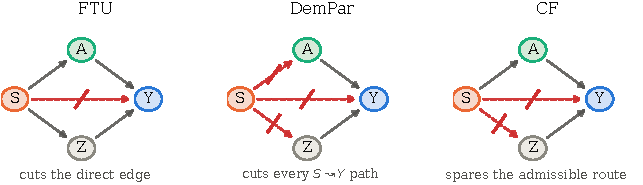
\includegraphics[width=\textwidth]{figs/pruning.pdf}
  \caption{Three fairness definitions as three sets of severed edges, acting on
  the graph the data is \emph{generated} from, not on the model trained
  afterwards \textcolor{red}{for a downstream task}. $S$ is the protected attribute, $Y$ the outcome, $A$ an
  admissible attribute whose influence is deemed legitimate, and $Z$ an
  intermediate proxy. Dashed red edges are cut. DemPar removes every directed
  $S \rightsquigarrow Y$ path; CF removes only those that avoid $A$, so the
  route $S \rightarrow A \rightarrow Y$ survives.}
  \label{fig:pruning}
\end{figure}

% =====================================================================
\section{Porting the mechanisms}
\label{sec:method}
% =====================================================================

We implement FTU, DemPar and CF against one
interface\footnote{Anonymized code, with instructions to reproduce every run
and table: \url{https://anonymous.4open.science/r/CausalFairnessInSDG-55EC/}.}
and attach it to nine generators from three unrelated families. The fairness definitions do not change; only
the graph the cut applies to does, and whether that graph is directed or
undirected.

\martine{If you use active voice in this paragraph, then it will be clearer that you are proposing these extended methods. Otherwise it may come across as if you are still describing existing work.}
\textbf{Marginals-based} synthesizers (MST, PrivBayes, PrivSyn, \martine{It may not be so simple for readers to see which papers these methods come from; maybe you can make that link in the paragraph ``The gap'' in Sec.~3. It may also be ok to change the citation format to numbers between square brackets to save space in the running text every time you cite a paper.} and
AIM\footnote{AIM \citep{mckenna2022aim} was ported after the main sweep and
run at $\varepsilon{=}1$ with one seed per (dataset, mechanism); it is
included as a smoke-test on a fourth marginals backbone, not pooled into the
Table~\ref{tab:fairness} averages.} \martine{Are the results for AIM reported anywhere in this paper? If not, maybe you can omit AIM here?} \s{Maybe we could specify it here which six. And then in the figures / tables, put a dagger next to the methods that are DP (and mention what the  dagger means in the caption)} \s{agreed, that this footnote need not be here --- it complicates the story. Just keep AIM mentioned in the list and just have a footnote attached to it saying that we only study AIM in the angelozzi2026where comparison, not the headline experiments. Dont need to mention seed, num trials, smoke-test, etc.}) form a
graphical model whose edges are the pairs of columns whose noisy joint counts
the synthesizer chooses to measure under the privacy budget; the release is
drawn from a distribution that reproduces those counts. Because the graph is
undirected, \hl{the fairness cut is enforced} \martine{``we enforce the fairness cut''} \s{Very much agreed. Look for opportunities throughout to follow this pattern where our work addresses the gap, which will help the reader know what was our contribution.} on paths rather than on ordered
parent$\rightarrow$child edges: whether adding a candidate pair would create
a forbidden $S$-to-$Y$ path depends on what is already in the model, so the
constraint is checked incrementally at each selection step. A pair the cut
excludes is never measured, making the constraint free in the privacy
accounting rather than merely cheap.\footnote{The freed $\varepsilon$ does
not buy the release a better fit. MST fixes its per-round budget from the
number of edges a spanning tree needs, before selection begins, so pruning
candidates shrinks each round's pool rather than enriching what remains, and
matched-pair $2$-way \hl{TVD} \martine{need to say first what TVD is} is worse under the cut, by $0.008$ for DemPar,
$0.003$ for CF and $0.001$ for FTU on Adult (ordered by how much structure
each removes).} \textbf{Causal GANs} (DECAF, plus CTGAN-based
\citep{xu2019ctgan} and DP-SGD \citep{abadi2016dpsgd} variants) \hl{use DECAF's
surrogate substitution unchanged,} \martine{switch to active voice} on the directed DAG. \textbf{Causal
diffusion} keeps the same factorisation and replaces each sub-network with a
small denoiser trained by supervised noise prediction; the cut is the same
code path, because what exposes an edge is that $X_i$ has its own network
reading only $\mathrm{pa}(X_i)$, true whether that network is trained
adversarially \textcolor{red}{as in GAN approaches} or by denoising.

\paragraph{Experimental setup.}
Two datasets, Adult \citep{becker1996adult} and COMPAS
\citep{angwin2016machinebias}; nine generators; four mechanisms
(\textsc{none}/FTU/DemPar/CF); $\varepsilon \in \{1,10,1000\}$ at $\delta =
10^{-9}$ for the \hl{six generators carrying a differential-privacy guarantee} \martine{I am not 100\% sure which of the generators are with DP. From Figure 2, is it the 3 marginals-based SDGs, and the ones that have DP in the name?}
\citep{dwork2006calibrating}; three protected/admissible role splits per
dataset; five seeds; 2{,}520 completed runs. One Adult split reproduces
DECAF's own setup (protected \texttt{sex}; admissible \texttt{occupation},
\texttt{hours-per-week}, \texttt{workclass}, \texttt{education}), one
follows PreFair's Table~1, and \hl{one is deliberately strict;} \martine{Not sure what ``deliberately strict'' means exactly. Remember that you should aim to give sufficient details to allow others to reproduce your results (I understand that such details are in the code that you release though).} COMPAS is absent
from DECAF's evaluation, so its splits follow PreFair and \hl{two variants} \martine{Similar comment as above: not enough info for reproducibility of the experiments} \s{agreed, I don't think it's obvious what the protected, outcome, admissable attributes are in settings we trialed. Maybe a small table would be helpful for this.}. For
the causal GAN and diffusion families the DAG for each dataset is specified
by hand from domain knowledge, as is standard in this literature (following
\citet{kusner2017counterfactual} and \citet{zhang2017causalframework}) and
held fixed across generators so effects are attributable to the mechanism.
The marginals-based generators choose their own undirected graph under the
privacy budget, and the cut is enforced on that graph.

\paragraph{Metrics.}
\emph{Fidelity} is \hl{$1$-way} \martine{Do you report the 1-way anywhere?} \s{valid point. I don't think we do report this. I'm pretty skeptical about having only reported one fidelity metric, which is not sufficient to show which generators are generally the best quality / fidelity. For example, there's also 1-way TVD, mean JSD, wasserstein distance (modified, found implemented in \url{https://github.com/steveng9/SyntheticData_MIA} , TSTR ratio (usefulness), correlation diff. etc. (these described and used in my other paper: \url{https://arxiv.org/pdf/2606.08372}) Can we concisely include at least one or two more to accompany 2-way TVD? This would help the reader contextualize the quality of the different generators, and why porting the fairness mechanism to marginals-based and diffusion-based is important. One small graphic could summarize all these, maybe with a star/radar chart for each of the three families, averaged over compas + adult, trials, generators in them, just epsilon=10 for the DP generators. We have several hours left before submission, so we have time to get more fidelity/quality measurements on the synthetic data. Maybe the edges of the radar plot can be 1 privacy metric, 1 or 2 fairness, and 3 quality/fidelity metrics? Instead of 3 radar plots, we could have one, with 3 polygons drawn (one for each family).} and $2$-way total-variation distance between the
synthetic and real marginals, averaged over columns and column-pairs (lower
is better; a value of $0$ means the synthetic and real marginals agree
exactly). \emph{Utility} is the test accuracy of an MLP trained on the
synthetic table to predict the outcome column (\texttt{income} on Adult,
\texttt{two\_year\_recid} on COMPAS) and evaluated on a real held-out $30\%$;
we report it as \emph{lift} over the majority-class rate so that a generator
with no learnable signal scores zero rather than the majority baseline.
\emph{Fairness} is that same MLP's worst-case demographic-parity gap across
values of the protected attribute, again evaluated against real held-out
people (DECAF's DF-\textsc{original} reference). Concretely, if $50\%$ of men
and $17\%$ of women in the released table are predicted to earn above
\$50k, the demographic-parity gap on Adult is $|0.50-0.17|=0.33$; a
mechanism that reduces it to $0.05$ has removed $85\%$ of the gap. \hl{We also
compute conditional parity and positive/negative-rate balance} \martine{I am not sure what those metrics are. Are their values reported anywhere in the paper?} \s{agreed. This is still very unclear / hard to get a grip on as a reader. Maybe we should explicitly make a dedicated definition of the feature fairness metric we use, how we refer to it, what it measures, formally, and then provide an example. Need to make clear why this is the best metric to showcase. 
Not buried in a paragraph about other fidelity / privacy metrics. Do we have a second fairness metric we report elsewhere? };  every claim
below reproduces on all four. Seed noise rivals the effects themselves
(median within-cell SD of the parity gap: $0.031$ on Adult, $0.092$ on
COMPAS), so every fairness number below is a \textbf{matched-pairs}
difference: each run with a fairness mechanism is differenced against the
run identical in dataset, generator, $\varepsilon$, role split \emph{and
seed} but with no fairness mechanism.

% =====================================================================
\section{Results}
\label{sec:results}
% =====================================================================

\begin{figure}[t]
  \centering
  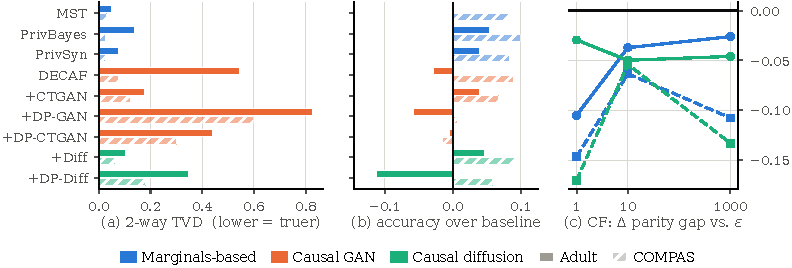
\includegraphics[width=\textwidth]{figs/results.pdf}
  \caption{\textbf{(a,\,b)} every generator with no fairness mechanism, averaged
  over $\varepsilon$, role splits and seeds; (a) $2$-way TVD to the real table
  (lower is better), (b) MLP lift over the majority-class rate (higher is
  better). A bar at zero in (b) means the data taught a classifier nothing, and
  a table with no signal has no disparity left to remove. \textbf{(c)} the
  matched-pairs reduction in parity gap from CF at each budget, for the two
  families present in every cell (marginals and diffusion; the causal GAN
  family lacks a matched cell at every budget because DP-GAN and DP-CTGAN
  collapse to a constant predictor in several cells). More negative is fairer,
  and the effect does not decay as $\varepsilon$ tightens. \martine{It wasn't simple for me to see the difference between the blue and the green lines in Fig.~2c on my print-out of the paper. If you could put a label/legend on each line in Fig.~2c, that would definitely help} \s{could we also add the porting graph back... That one was good (not necessarily part a needed, but something like the second part which clear shows differences in the 3 families.}}
  \label{fig:results}
\end{figure}

\subsection{Fidelity and utility}

Fidelity separates the nine generators cleanly (Figure~\ref{fig:results}a).
The marginals-based synthesizers dominate, as expected since they optimise
almost exactly $2$-way TVD: MST reaches $0.048$ on Adult and $0.030$ on
COMPAS. Diffusion is the next tier \s{again, doesn't this quality metric contradict the recent literature that diffusion has best tabular fidelity. Need to be more precise in such claims, that "our metric shows" or something like that, if this is unique to 2-way TVD, etc. which is just a very small window into actual, holistic fidelity.} and holds it at every privacy level: our
non-private diffusion \hl{port} \martine{What do you call it a ``port''? Is it because you use the DAG from DECAF again in the diffusion model?} reaches $0.103$ on Adult against DECAF's own
$0.544$, and with DP-SGD attached, DP-diffusion at $0.346$ still leads
DP-GAN at $0.439$ and DP-CTGAN at $0.830$.

Utility is the load-bearing panel for what follows (Figure~\ref{fig:results}b). \martine{What are the accuracies for train on real--test on real?}
Most generators clear the majority-class baseline meaningfully: on Adult
PrivBayes reaches $0.05$ lift over the $0.758$ majority-class rate \martine{So the accuracy becomes 0.808? I feel like you should say once explicitly that the accuracy when training on the synthetic data is 80\% because otherwise it may feel like $0.05$ is a tiny number.}, PrivSyn
$0.05$, our non-private diffusion port $0.04$, and DP-diffusion at
$\varepsilon\geq10$ sits just above baseline. \hl{Two cells are trouble:} \martine{Looking at Fig.~2b, DECAF, DP-CTGAN, and DP-Diff also have stuff on the left (i.e.~accuracies below the baseline); it's not so clear to me why you call out MST and DP-GAN as troublesome but not those other 3} \s{agreed. This isn't clear. The results in fig 2.b. seem a little all over the place, and maybe we need TSTR ratio, or need to redo the accuracy experiments with RF, or a different outcome / label feature? Seems very bizarre the a diffusion generator accuracy DP-diff is so far below baseline... Need to fix this, or report something else since there's no reasonable explanaition for it..} MST on
Adult sits at exactly zero lift (accuracy $0.747$, majority rate $0.758$),
and the DP-GAN family collapses to a constant predictor in several
$\varepsilon{=}1$ cells. A table that teaches a classifier nothing has no
disparity for a fairness mechanism to remove, and is scored as perfectly
fair by every existing fairness metric. Every fairness claim below is a
matched-pair difference holding the generator fixed, so this artefact does not
confound the mechanism's effect; it does mean an absolute fairness number is
uninterpretable without the utility number beside it for those two cells.

\subsection{Fairness: the definitions transfer, the magnitude does not}

\begin{table}[t]
  \caption{Matched-pairs change in the worst-case demographic-parity gap from
  applying each mechanism, pooled within generator family. \emph{end} is the
  gap that remains after the mechanism; $\Delta$\,gap is the mean paired
  change with a 95\% CI (negative = gap shrunk); $\Delta$\,acc is the paired
  MLP-accuracy change. Base (no-mechanism) gaps are in the family headers.}
  \label{tab:fairness}
  \centering
  \footnotesize
  \setlength{\tabcolsep}{5pt}
  \begin{tabular}{l ccc c ccc}
    \toprule
    & \multicolumn{3}{c}{\textbf{Adult}} & & \multicolumn{3}{c}{\textbf{COMPAS}} \\
    \cmidrule(lr){2-4} \cmidrule(lr){6-8}
    Mech. & end & $\Delta$\,gap & $\Delta$\,acc & & end & $\Delta$\,gap & $\Delta$\,acc \\
    \midrule
    \multicolumn{8}{l}{\textit{Marginals-based} (MST, PrivBayes, PrivSyn), base gap 0.143 / 0.331, $n=135$} \\
    FTU & 0.121 & $-0.022 \pm 0.020$ & $+0.002$ & & 0.254 & $-0.076 \pm 0.027$ & $+0.003$ \\
    CF  & 0.087 & $-0.056 \pm 0.020$ & $-0.005$ & & 0.225 & $-0.106 \pm 0.027$ & $-0.011$ \\
    DemPar & 0.071 & $-0.073 \pm 0.021$ & $-0.032$ & & 0.230 & $-0.101 \pm 0.029$ & $-0.033$ \\
    \addlinespace[2pt]
    \multicolumn{8}{l}{\textit{Causal GAN} (DECAF, +CTGAN, +DP-GAN, +DP-CTGAN), base gap 0.074 / 0.238, $n=102/96$} \\
    FTU & 0.072 & $-0.003 \pm 0.006$ & $-0.000$ & & 0.156 & $-0.081 \pm 0.028$ & $-0.002$ \\
    CF  & 0.019 & $-0.055 \pm 0.019$ & $-0.001$ & & 0.134 & $-0.103 \pm 0.031$ & $-0.017$ \\
    DemPar & 0.007 & $-0.068 \pm 0.021$ & $-0.003$ & & 0.094 & $-0.145 \pm 0.039$ & $-0.049$ \\
    \addlinespace[2pt]
    \multicolumn{8}{l}{\textit{Causal diffusion} (DECAF+Diffusion, +DP-Diffusion), base gap 0.069 / 0.294, $n=60$} \\
    FTU & 0.059 & $-0.010 \pm 0.014$ & $-0.004$ & & 0.193 & $-0.101 \pm 0.029$ & $-0.013$ \\
    CF  & 0.015 & $-0.055 \pm 0.017$ & $-0.015$ & & 0.160 & $-0.134 \pm 0.034$ & $-0.033$ \\
    DemPar & 0.003 & $-0.066 \pm 0.016$ & $-0.007$ & & 0.126 & $-0.167 \pm 0.034$ & $-0.088$ \\
    \bottomrule
  \end{tabular}

  \martine{What are the $n=135$ etc. values listed in this table?} \s{agreed that this is confusing and not a necessary detail.}

  \martine{I would have found it clearer to see actual accuracy values (in addition to accuracy gaps) in this table. Just like you have an ``end'' column for the demographic parity gap, can you include a column for the final accuracy?}
\end{table}


\textbf{The definitions transfer.} In every generator family, on both
datasets and at every privacy level, cutting edges reduces the downstream
parity gap (Table~\ref{tab:fairness}: the mean matched-pair reductions are
every one signed the same way and every one comfortably outside its own
$95\%$ interval). This answers DECAF's own conjecture in the sense that
matters first: nothing about the three definitions requires a GAN, and
nothing about them requires a supplied directed DAG.

\textbf{The magnitude does not transfer, and the pooled averages hide that.}
The pooled numbers look invariant at first: on Adult, CF's mean matched-pair
reduction in parity gap is $0.056 \pm 0.020$ on marginals, $0.055 \pm 0.019$
on causal GANs and $0.055 \pm 0.017$ on causal diffusion, three means
\hl{agreeing to $0.002$} \martine{do you mean ``agreeing to $0.055$''?}. The per-generator effects on Adult span $0.002$ (MST)
to $0.173$ (DECAF), and each family happens to contain both a generator
that reproduces the disparity in full and one whose signal has collapsed to
the majority class (Figure~\ref{fig:results}b), so the family means average
across those extremes onto the same intermediate value. The comparison as a fraction of
each generator's own baseline parity gap is more informative. Restricted to
matched pairs where there is disparity to remove (baseline gap $>0.05$) and
where the generator learned something (lift $>0.02$), CF removes $89\%$ of
the baseline parity gap on the causal diffusion family, $75\%$ on the causal
GAN family and $29\%$ on the marginals-based family on Adult ($43\%$, $32\%$
and $22\%$ on COMPAS). Concretely, on DECAF
diffusion under DemPar on Adult, the fraction of men in the released table
that the downstream classifier predicts to earn above \$50k differs from the
corresponding fraction for women by $0.29$ before the mechanism is applied
and $0.03$ after. On MST the same mechanism moves it from $0.11$ to $0.09$.
Variance partitioning confirms the split: which family the generator belongs
to explains essentially none of the raw reduction ($\eta^2 = 0.00$) and
about a quarter of the fraction removed ($\eta^2 = 0.25$; $n = 432$ matched
pairs in the disparity-and-signal subset).

\textbf{The gap has a structural cause: the same definition compiles to two
operations on very different graphs.} The causal GAN and diffusion families
receive a directed DAG from a domain expert and sever its edges by surrogate
substitution at sampling time. A marginals-based synthesizer receives no DAG;
it selects an undirected structure under the privacy budget, so the definition
is enforced during that selection and can only sever an edge the structure
already carries. The two graphs carry very different amounts of
protected-to-outcome dependence (Table~\ref{tab:edges}): the hand-designed
Adult DAG puts $\approx 9$ edges on some $S$-to-$Y$ path that DemPar must
sever, whereas the private, sparse marginals graph offers only $4$. So the GAN
and diffusion families cut more edges in absolute terms but a smaller fraction
of their already-small baseline disparity, while the marginals family cuts
fewer edges but a much larger fraction of its gap.

\begin{table}[t]
  \caption{Mean number of edges the mechanism must sever, per run, per
  generator family. For the causal GAN/diffusion families the count is
  deterministic: it is the number of DAG edges DECAF's surrogate
  substitution would replace given each dataset's role split. For marginals
  it is the minimum edge cut needed on the baseline (no-mechanism) learned
  undirected graph to break every forbidden $S$-to-$Y$ path (paths through
  admissibles are legal under CF, hence its intermediate size). DemPar
  $\geq$ CF $\geq$ FTU by construction.}
  \label{tab:edges}
  \centering
  \footnotesize
  \setlength{\tabcolsep}{6pt}
  \begin{tabular}{l ccc c ccc}
    \toprule
    & \multicolumn{3}{c}{\textbf{Adult}} & & \multicolumn{3}{c}{\textbf{COMPAS}} \\
    \cmidrule(lr){2-4} \cmidrule(lr){6-8}
    Family & FTU & CF & DemPar & & FTU & CF & DemPar \\
    \midrule
    Causal GAN / diffusion (fixed DAG) & 0.75 & 4.00 & 8.75 & & 1.33 & 1.67 & 3.33 \\
    Marginals-based (learned graph)   & 0.58 & 2.81 & 4.24 & & 0.96 & 2.27 & 3.72 \\
    \bottomrule
  \end{tabular}
\end{table}

\textbf{The predicted ordering falls out of the data.} Ranked by parity gap
left behind, \textsc{none} $>$ FTU $>$ CF $>$ DemPar holds in five of six
(dataset $\times$ family) cells (Table~\ref{tab:fairness}). CF landing
between the other two is a substantive check on the mechanism, not a
formality: CF spares disparity routed through the admissible attribute, so
wherever the role split gives DemPar a mediator to cut and CF one to spare,
CF must recover strictly less reduction, and it does wherever the two
separate by more than seed noise.

\textbf{Fairness through unawareness is weak, and on Adult barely acts.}
Pooled over Adult, FTU shifts the matched-pair parity gap by only $0.013$
on average. The pooled figure is the sum of two very different behaviours:
on MST the mechanism is a literal no-op in all $45$ Adult pairs, because
the direct protected-to-income marginal is one the private structure search
never buys under our budgets and there is nothing for the filter to
exclude; on the GAN and diffusion families FTU does cut, but the influence
promptly re-routes through proxy attributes. This is the textbook criticism
of unawareness, confirmed constructively: the cheap cut fails where the two
path-based cuts, on the same generators and seeds, work.

\textbf{The utility cost tracks the aggressiveness of the cut}, and is modest
for the cuts worth making: pooled over Adult, DemPar costs $1.7$ accuracy
points and CF costs $0.6$; on COMPAS, $5.0$ and $1.7$. CF stays under two
accuracy points in five of six (dataset $\times$ family) cells.

\subsection{How this compares to intervening downstream}

\begin{table}[t]
\centering\footnotesize
\caption{\textbf{Where to intervene, on identical data.} MST synthetic
training data, real held-out test set, XGBoost, 5 seeds, all inside the
benchmark code of \citet{angelozzi2026where}. Entries are $|$parity
gap$|$\,/\,accuracy; \textbf{bold} marks the best value in each column at
the displayed precision (lower gap, higher accuracy; ties bolded together).
The eight comparison mitigators act on the released table or on the model
trained from it; our three (\textbf{in-gen (ours)}) act inside the
generator. Majority-class accuracy is $0.758$ (Adult) and $0.533$ (COMPAS),
so learned fair representations buy their low gap by falling to it. \martine{What is the point of releasing synthetic data, if the downstream model has the same accuracy or is worse than the baseline?}}
\label{tab:baselines}
\begin{tabular}{llcccc}
\toprule
 & & \multicolumn{2}{c}{Adult} & \multicolumn{2}{c}{COMPAS} \\
\cmidrule(lr){3-4}\cmidrule(lr){5-6}
stage & intervention & $\varepsilon{=}1$ & $\varepsilon{=}10$ & $\varepsilon{=}1$ & $\varepsilon{=}10$ \\
\midrule
 & no mitigation        & 0.068 / 0.74 & 0.073 / 0.74 & 0.109 / \textbf{0.61} & 0.190 / 0.61 \\
\addlinespace[2pt]
pre  & Reweighing         & 0.087 / \textbf{0.75} & 0.085 / \textbf{0.75} & 0.132 / \textbf{0.61} & 0.093 / 0.61 \\
pre  & Disp.\ impact rem. & 0.078 / 0.74 & 0.105 / 0.72 & 0.119 / \textbf{0.61} & 0.205 / \textbf{0.62} \\
pre  & Learned fair repr. & 0.018 / 0.72 & 0.031 / 0.70 & 0.037 / 0.50 & 0.028 / 0.51 \\
\addlinespace[2pt]
in   & Exp.\ gradient     & 0.047 / 0.74 & 0.058 / 0.74 & 0.115 / \textbf{0.61} & 0.053 / 0.60 \\
in   & Grid search        & 0.068 / 0.74 & 0.073 / 0.74 & 0.109 / \textbf{0.61} & 0.190 / 0.61 \\
\addlinespace[2pt]
post & Reject option      & 0.045 / 0.60 & 0.046 / 0.61 & 0.045 / 0.56 & 0.046 / 0.54 \\
post & Equalised odds     & \textbf{0.009} / 0.71 & 0.015 / 0.72 & \textbf{0.024} / 0.58 & \textbf{0.023} / 0.59 \\
post & Calib.\ eq.\ odds  & 0.049 / \textbf{0.75} & 0.040 / \textbf{0.75} & 0.485 / 0.56 & 0.415 / 0.57 \\
\addlinespace[2pt]
\textbf{in-gen (ours)} & FTU    & 0.073 / 0.74 & 0.062 / 0.74 & 0.087 / 0.53 & 0.155 / 0.61 \\
\textbf{in-gen (ours)} & DemPar & 0.010 / \textbf{0.75} & \textbf{0.006} / \textbf{0.75} & 0.067 / 0.53 & 0.148 / \textbf{0.62} \\
\textbf{in-gen (ours)} & CF     & 0.015 / \textbf{0.75} & 0.029 / 0.74 & 0.111 / 0.59 & 0.155 / 0.61 \\
\bottomrule
\end{tabular}
\end{table}


Everything so far measures the mechanism against itself. To place it against
the alternatives an institution actually has, we ran the benchmark of
\citet{angelozzi2026where} (introduced in \S\ref{sec:related}), which asks
where in a differentially private synthetic pipeline a fairness intervention
should go and offers eight standard answers spread across pre-processing the
table, constraining the \textcolor{red}{downstream} classifier, and post-processing its predictions. We
add ours as a fourth stage, applied inside the generator. We use their code
unmodified (their preprocessed data, splits, MST synthesizer, XGBoost
classifier and aif360 metrics); the only change is that our arm's training
table comes from our MST under FTU, DemPar or CF rather than theirs.
Table~\ref{tab:baselines} is the result.

On Adult the in-generator cut is on the fairness/accuracy frontier
(Table~\ref{tab:baselines}, columns 1--2). DemPar in-generator leaves a
parity gap of $0.010$ at $0.748$ accuracy; the only downstream mitigator that
reaches a comparable gap is equalized-odds post-processing (which threshold-
shifts the classifier per group) at $0.009$, and it costs $3.4$ more accuracy
points to get there. Reweighing and the disparate-impact remover leave the
release \emph{less} fair than no mitigation at all in this cell, and grid
search is an exact no-op. On COMPAS the ordering reverses: post-processing
reaches $0.023$ where our best cut reaches $0.148$. This is the same finding
as \S\ref{sec:results} seen from outside, since at these budgets the
privately selected MST structure barely encodes the protected-to-outcome
dependence and there is correspondingly little for a cut to sever, whereas a
mitigator acting on the trained \st{model} \textcolor{red}{downstream classifier} is not subject to that limit. FTU and
CF are exact no-ops on Adult in this harness too, reproducing the FTU result
above in a different codebase and metric.

This is not a like-for-like ranking of techniques: a downstream mitigator is
applied by whoever trains a model, whereas the in-generator cut is applied once
by the synthetic data publisher and is the only one of the four that ships with the released
table (Sec.~\ref{sec:discussion}).

\subsection{Privacy and fairness are nearly independent}

\hl{The standard expectation for privacy and fairness is a trade-off:
differential privacy has been shown to fall hardest on the smallest groups} \s{yes, I think this isn't really an accurate depiction of the bagdasaryan2019disparate (i.e. "Eugene's paper"); maybe make clear that differential privacy causes the \textit{accuracy} to fall hardest.}
\citep{bagdasaryan2019disparate}, \hl{so tightening $\varepsilon$ should both
widen the parity gap in the released table and blunt any attempt to close
it.} \martine{Eugene's paper is about the fact that a classifier trained with DP-SGD is less accurate for instances from minority classes that occur less frequently in the data. That is to be expected, because DP suppresses outliers/special cases (in an attempt to hide them in the crowd), so the resulting model will not be so accurate for these outliers/special cases. What you measure with the ``demographic parity gap'' is something quite different. You want a classifier to predict a class label with the same probability for members from a protected group as for members from a non-protected group (regardless whether that prediction is correct or not). I do not think that Eugene's findings necessarily transfer to this case. It's not even clear to me whether what you have as protected members in your experiments are minority groups in the data.} \s{I agree. We need to make clear what the the features and groups are. Also, the citation from bagdasaryan2019disparate needs to be discussed in such a way that results about DP like this one might simply lead to suspician that increasing DP also reduces fairness for minority groups (some sort of loss of benefit is the point), but we find here that this is not the case? Something like that? Should be kept simple and precise. } In this setting we do not see the second half. Cutting edges reduces
the parity gap at least as much at the strong $\varepsilon{=}1$ as at the
permissive $\varepsilon{=}1000$ in nine of twelve (family $\times$ dataset
$\times$ \{CF, DemPar\}) cells; two of the three exceptions are COMPAS GAN
cells where the backbone has already collapsed to a constant predictor at
$\varepsilon{=}1$ and has no disparity left to remove. For marginals-based
generators on Adult, CF's mean paired reduction in parity gap is $0.105$ at
$\varepsilon{=}1$ against $0.026$ at $\varepsilon{=}1000$ (on COMPAS, $0.147$
against $0.108$). \hl{DP noise widens the baseline gap at $\varepsilon{=}1$,} \martine{How much is that widening? I am not sure if you report those numbers anywhere here? And how do you explain it?}
leaving more to remove, but that is not the whole story: the reduction moves
the same way as a fraction of baseline ($68\%$ against $18\%$ on Adult). For
causal diffusion it is essentially flat ($0.030$, $0.050$, $0.046$ across the
three budgets on Adult). One deviation we cannot yet explain
(Figure~\ref{fig:results}c): \hl{the effect at $\varepsilon{=}10$ is weaker than
at either neighbour in both families and both datasets.} \martine{I see that for COMPAS but not for Adult?} \s{If i read the graph correctly, we see this for 3 of the 4 lines drawn (i.e. 2/2 compas, and 1/2 adult, right? I think the "the effect at $\varepsilon{=}10$ is weaker than
at either neighbour" is worded poorly, and it isn't clear what that means.}

\textbf{One private generator fails outright}, on a claim DECAF makes. DECAF
argues from the post-processing theorem that it ``can be directly used for
generating private synthetic data by replacing the standard discriminator by
a differentially private discriminator.'' The accounting is correct; the
output is not. Attaching DP-SGD \citep{abadi2016dpsgd} to DECAF's WGAN-GP
critic in this way (the DP-GAN row in Table~\ref{tab:fairness}) collapses
the synthetic outcome to a single class in $168$ of $360$ runs ($47\%$),
every COMPAS run at $\varepsilon{=}1$ included. Two independent changes each
remove the failure: substituting a CTGAN representation under the same
adversarial training ($1/360$), and substituting diffusion for the WGAN-GP
critic under DECAF's own representation ($0/360$). Two unrelated repairs
locate the cause in DP-SGD on a weight-clipped critic, not in private causal
generation as such.

% =====================================================================
\section{Discussion}
\label{sec:discussion}
% =====================================================================
\wkDiscussion

\bibliographystyle{plainnat}
\bibliography{refs}

\section*{NeurIPS Paper Checklist}

\begin{enumerate}

\item {\bf Claims}
    \item[] Question: Do the main claims made in the abstract and introduction accurately reflect the paper's contributions and scope?
    \item[] Answer: \answerYes{}
    \item[] Justification: The abstract and introduction claim that DECAF's edge-surgery fairness mechanism ports beyond its original GAN to marginals-based and diffusion generators; Sections~\ref{sec:method}--\ref{sec:results} establish exactly this across nine generators, two datasets and three privacy budgets, and we are explicit that the \emph{magnitude} of the effect does not transfer even though the definitions do.
    \item[] Guidelines:
    \begin{itemize}
        \item The answer \answerNA{} means that the abstract and introduction do not include the claims made in the paper.
        \item The abstract and/or introduction should clearly state the claims made, including the contributions made in the paper and important assumptions and limitations. A \answerNo{} or \answerNA{} answer to this question will not be perceived well by the reviewers.
        \item The claims made should match theoretical and experimental results, and reflect how much the results can be expected to generalize to other settings.
        \item It is fine to include aspirational goals as motivation as long as it is clear that these goals are not attained by the paper.
    \end{itemize}

\item {\bf Limitations}
    \item[] Question: Does the paper discuss the limitations of the work performed by the authors?
    \item[] Answer: \answerYes{}
    \item[] Justification: Limitations are discussed inline rather than in a separate section: the effect magnitude does not transfer across families and depends on the supplied or privately learned graph (\S\ref{sec:results}); two generators produce degenerate-utility tables that trivially appear fair (\S\ref{sec:results}); the reduction at $\varepsilon{=}10$ is weaker than at either neighbouring budget and we cannot yet explain it (\S\ref{sec:results}); and the causal-GAN/diffusion results rely on a hand-specified DAG (\S\ref{sec:method}).
    \item[] Guidelines:
    \begin{itemize}
        \item The answer \answerNA{} means that the paper has no limitation while the answer \answerNo{} means that the paper has limitations, but those are not discussed in the paper.
        \item The authors are encouraged to create a separate ``Limitations'' section in their paper.
        \item The paper should point out any strong assumptions and how robust the results are to violations of these assumptions (e.g., independence assumptions, noiseless settings, model well-specification, asymptotic approximations only holding locally). The authors should reflect on how these assumptions might be violated in practice and what the implications would be.
        \item The authors should reflect on the scope of the claims made, e.g., if the approach was only tested on a few datasets or with a few runs. In general, empirical results often depend on implicit assumptions, which should be articulated.
        \item The authors should reflect on the factors that influence the performance of the approach. For example, a facial recognition algorithm may perform poorly when image resolution is low or images are taken in low lighting. Or a speech-to-text system might not be used reliably to provide closed captions for online lectures because it fails to handle technical jargon.
        \item The authors should discuss the computational efficiency of the proposed algorithms and how they scale with dataset size.
        \item If applicable, the authors should discuss possible limitations of their approach to address problems of privacy and fairness.
        \item While the authors might fear that complete honesty about limitations might be used by reviewers as grounds for rejection, a worse outcome might be that reviewers discover limitations that aren't acknowledged in the paper. The authors should use their best judgment and recognize that individual actions in favor of transparency play an important role in developing norms that preserve the integrity of the community. Reviewers will be specifically instructed to not penalize honesty concerning limitations.
    \end{itemize}

\item {\bf Theory assumptions and proofs}
    \item[] Question: For each theoretical result, does the paper provide the full set of assumptions and a complete (and correct) proof?
    \item[] Answer: \answerNA{}
    \item[] Justification: The paper makes no formal theoretical claims and states no theorems; all results are empirical.
    \item[] Guidelines:
    \begin{itemize}
        \item The answer \answerNA{} means that the paper does not include theoretical results.
        \item All the theorems, formulas, and proofs in the paper should be numbered and cross-referenced.
        \item All assumptions should be clearly stated or referenced in the statement of any theorems.
        \item The proofs can either appear in the main paper or the supplemental material, but if they appear in the supplemental material, the authors are encouraged to provide a short proof sketch to provide intuition.
        \item Inversely, any informal proof provided in the core of the paper should be complemented by formal proofs provided in appendix or supplemental material.
        \item Theorems and Lemmas that the proof relies upon should be properly referenced.
    \end{itemize}

    \item {\bf Experimental result reproducibility}
    \item[] Question: Does the paper fully disclose all the information needed to reproduce the main experimental results of the paper to the extent that it affects the main claims and/or conclusions of the paper (regardless of whether the code and data are provided or not)?
    \item[] Answer: \answerYes{}
    \item[] Justification: Section~\ref{sec:method} specifies the datasets, generators, fairness mechanisms, privacy budgets, role splits, seed count, downstream classifier and matched-pairs protocol, and we release an anonymized code repository with instructions to reproduce every run and every table (footnote in \S\ref{sec:method}).
    \item[] Guidelines:
    \begin{itemize}
        \item The answer \answerNA{} means that the paper does not include experiments.
        \item If the paper includes experiments, a \answerNo{} answer to this question will not be perceived well by the reviewers: Making the paper reproducible is important, regardless of whether the code and data are provided or not.
        \item If the contribution is a dataset and\slash or model, the authors should describe the steps taken to make their results reproducible or verifiable.
        \item Depending on the contribution, reproducibility can be accomplished in various ways. For example, if the contribution is a novel architecture, describing the architecture fully might suffice, or if the contribution is a specific model and empirical evaluation, it may be necessary to either make it possible for others to replicate the model with the same dataset, or provide access to the model. In general. releasing code and data is often one good way to accomplish this, but reproducibility can also be provided via detailed instructions for how to replicate the results, access to a hosted model (e.g., in the case of a large language model), releasing of a model checkpoint, or other means that are appropriate to the research performed.
        \item While NeurIPS does not require releasing code, the conference does require all submissions to provide some reasonable avenue for reproducibility, which may depend on the nature of the contribution. For example
        \begin{enumerate}
            \item If the contribution is primarily a new algorithm, the paper should make it clear how to reproduce that algorithm.
            \item If the contribution is primarily a new model architecture, the paper should describe the architecture clearly and fully.
            \item If the contribution is a new model (e.g., a large language model), then there should either be a way to access this model for reproducing the results or a way to reproduce the model (e.g., with an open-source dataset or instructions for how to construct the dataset).
            \item We recognize that reproducibility may be tricky in some cases, in which case authors are welcome to describe the particular way they provide for reproducibility. In the case of closed-source models, it may be that access to the model is limited in some way (e.g., to registered users), but it should be possible for other researchers to have some path to reproducing or verifying the results.
        \end{enumerate}
    \end{itemize}


\item {\bf Open access to data and code}
    \item[] Question: Does the paper provide open access to the data and code, with sufficient instructions to faithfully reproduce the main experimental results, as described in supplemental material?
    \item[] Answer: \answerYes{}
    \item[] Justification: Both datasets (Adult, COMPAS) are public, and we release an anonymized code repository with the synthesizer/mechanism implementations and the run and analysis scripts at \url{https://anonymous.4open.science/r/CausalFairnessInSDG-55EC/} (also cited in \S\ref{sec:method}).
    \item[] Guidelines:
    \begin{itemize}
        \item The answer \answerNA{} means that paper does not include experiments requiring code.
        \item Please see the NeurIPS code and data submission guidelines (\url{https://neurips.cc/public/guides/CodeSubmissionPolicy}) for more details.
        \item While we encourage the release of code and data, we understand that this might not be possible, so \answerNo{} is an acceptable answer. Papers cannot be rejected simply for not including code, unless this is central to the contribution (e.g., for a new open-source benchmark).
        \item The instructions should contain the exact command and environment needed to run to reproduce the results. See the NeurIPS code and data submission guidelines (\url{https://neurips.cc/public/guides/CodeSubmissionPolicy}) for more details.
        \item The authors should provide instructions on data access and preparation, including how to access the raw data, preprocessed data, intermediate data, and generated data, etc.
        \item The authors should provide scripts to reproduce all experimental results for the new proposed method and baselines. If only a subset of experiments are reproducible, they should state which ones are omitted from the script and why.
        \item At submission time, to preserve anonymity, the authors should release anonymized versions (if applicable).
        \item Providing as much information as possible in supplemental material (appended to the paper) is recommended, but including URLs to data and code is permitted.
    \end{itemize}


\item {\bf Experimental setting/details}
    \item[] Question: Does the paper specify all the training and test details (e.g., data splits, hyperparameters, how they were chosen, type of optimizer) necessary to understand the results?
    \item[] Answer: \answerYes{}
    \item[] Justification: Section~\ref{sec:method} gives the datasets, the $30\%$ real held-out test split, the downstream MLP, the three protected/admissible role splits, the privacy budgets ($\varepsilon \in \{1,10,1000\}$, $\delta = 10^{-9}$) and five seeds per cell; the remaining hyperparameters are fixed in the released code.
    \item[] Guidelines:
    \begin{itemize}
        \item The answer \answerNA{} means that the paper does not include experiments.
        \item The experimental setting should be presented in the core of the paper to a level of detail that is necessary to appreciate the results and make sense of them.
        \item The full details can be provided either with the code, in appendix, or as supplemental material.
    \end{itemize}

\item {\bf Experiment statistical significance}
    \item[] Question: Does the paper report error bars suitably and correctly defined or other appropriate information about the statistical significance of the experiments?
    \item[] Answer: \answerYes{}
    \item[] Justification: Every fairness number is a matched-pairs difference (each mechanism run is differenced against the no-mechanism run identical in dataset, generator, budget, role split and seed); Table~\ref{tab:fairness} reports mean paired changes with $95\%$ confidence intervals, and \S\ref{sec:method} reports the within-cell seed standard deviation that motivates the paired design.
    \item[] Guidelines:
    \begin{itemize}
        \item The answer \answerNA{} means that the paper does not include experiments.
        \item The authors should answer \answerYes{} if the results are accompanied by error bars, confidence intervals, or statistical significance tests, at least for the experiments that support the main claims of the paper.
        \item The factors of variability that the error bars are capturing should be clearly stated (for example, train/test split, initialization, random drawing of some parameter, or overall run with given experimental conditions).
        \item The method for calculating the error bars should be explained (closed form formula, call to a library function, bootstrap, etc.)
        \item The assumptions made should be given (e.g., Normally distributed errors).
        \item It should be clear whether the error bar is the standard deviation or the standard error of the mean.
        \item It is OK to report 1-sigma error bars, but one should state it. The authors should preferably report a 2-sigma error bar than state that they have a 96\% CI, if the hypothesis of Normality of errors is not verified.
        \item For asymmetric distributions, the authors should be careful not to show in tables or figures symmetric error bars that would yield results that are out of range (e.g., negative error rates).
        \item If error bars are reported in tables or plots, the authors should explain in the text how they were calculated and reference the corresponding figures or tables in the text.
    \end{itemize}

\item {\bf Experiments compute resources}
    \item[] Question: For each experiment, does the paper provide sufficient information on the computer resources (type of compute workers, memory, time of execution) needed to reproduce the experiments?
    \item[] Answer: \answerYes{}
    \item[] Justification: All experiments run on a single shared Linux workstation; the models are small (tabular MLPs and per-column generators/denoisers), a single GPU is used for the GAN and diffusion backbones, and the full 2{,}520-run sweep completes in roughly 6--12 hours of wall-clock time when parallelised.
    \item[] Guidelines:
    \begin{itemize}
        \item The answer \answerNA{} means that the paper does not include experiments.
        \item The paper should indicate the type of compute workers CPU or GPU, internal cluster, or cloud provider, including relevant memory and storage.
        \item The paper should provide the amount of compute required for each of the individual experimental runs as well as estimate the total compute.
        \item The paper should disclose whether the full research project required more compute than the experiments reported in the paper (e.g., preliminary or failed experiments that didn't make it into the paper).
    \end{itemize}

\item {\bf Code of ethics}
    \item[] Question: Does the research conducted in the paper conform, in every respect, with the NeurIPS Code of Ethics \url{https://neurips.cc/public/EthicsGuidelines}?
    \item[] Answer: \answerYes{}
    \item[] Justification: The research uses only public, widely studied benchmark datasets, involves no human-subjects data collection, and its goal (reducing demographic disparity in released synthetic data under privacy guarantees) is consistent with the NeurIPS Code of Ethics.
    \item[] Guidelines:
    \begin{itemize}
        \item The answer \answerNA{} means that the authors have not reviewed the NeurIPS Code of Ethics.
        \item If the authors answer \answerNo, they should explain the special circumstances that require a deviation from the Code of Ethics.
        \item The authors should make sure to preserve anonymity (e.g., if there is a special consideration due to laws or regulations in their jurisdiction).
    \end{itemize}


\item {\bf Broader impacts}
    \item[] Question: Does the paper discuss both potential positive societal impacts and negative societal impacts of the work performed?
    \item[] Answer: \answerYes{}
    \item[] Justification: The intended impact is positive: enabling institutions to remove unfair pathways from synthetic releases (Introduction, Discussion). We also flag concrete failure modes: a generator that teaches a classifier nothing has no disparity to remove yet scores as perfectly fair, so a fairness number is uninterpretable without its utility number (\S\ref{sec:results}), and an in-generator cut can give false assurance if downstream consumers assume more disparity was removed than the graph actually permitted (\S\ref{sec:results}, Discussion).
    \item[] Guidelines:
    \begin{itemize}
        \item The answer \answerNA{} means that there is no societal impact of the work performed.
        \item If the authors answer \answerNA{} or \answerNo, they should explain why their work has no societal impact or why the paper does not address societal impact.
        \item Examples of negative societal impacts include potential malicious or unintended uses (e.g., disinformation, generating fake profiles, surveillance), fairness considerations (e.g., deployment of technologies that could make decisions that unfairly impact specific groups), privacy considerations, and security considerations.
        \item The conference expects that many papers will be foundational research and not tied to particular applications, let alone deployments. However, if there is a direct path to any negative applications, the authors should point it out. For example, it is legitimate to point out that an improvement in the quality of generative models could be used to generate Deepfakes for disinformation. On the other hand, it is not needed to point out that a generic algorithm for optimizing neural networks could enable people to train models that generate Deepfakes faster.
        \item The authors should consider possible harms that could arise when the technology is being used as intended and functioning correctly, harms that could arise when the technology is being used as intended but gives incorrect results, and harms following from (intentional or unintentional) misuse of the technology.
        \item If there are negative societal impacts, the authors could also discuss possible mitigation strategies (e.g., gated release of models, providing defenses in addition to attacks, mechanisms for monitoring misuse, mechanisms to monitor how a system learns from feedback over time, improving the efficiency and accessibility of ML).
    \end{itemize}

\item {\bf Safeguards}
    \item[] Question: Does the paper describe safeguards that have been put in place for responsible release of data or models that have a high risk for misuse (e.g., pre-trained language models, image generators, or scraped datasets)?
    \item[] Answer: \answerNA{}
    \item[] Justification: The paper releases fairness-mechanism code operating on public tabular benchmarks; it releases no pre-trained generative model, scraped dataset, or other artifact with a high risk for misuse.
    \item[] Guidelines:
    \begin{itemize}
        \item The answer \answerNA{} means that the paper poses no such risks.
        \item Released models that have a high risk for misuse or dual-use should be released with necessary safeguards to allow for controlled use of the model, for example by requiring that users adhere to usage guidelines or restrictions to access the model or implementing safety filters.
        \item Datasets that have been scraped from the Internet could pose safety risks. The authors should describe how they avoided releasing unsafe images.
        \item We recognize that providing effective safeguards is challenging, and many papers do not require this, but we encourage authors to take this into account and make a best faith effort.
    \end{itemize}

\item {\bf Licenses for existing assets}
    \item[] Question: Are the creators or original owners of assets (e.g., code, data, models), used in the paper, properly credited and are the license and terms of use explicitly mentioned and properly respected?
    \item[] Answer: \answerYes{}
    \item[] Justification: Every existing asset is cited to its original source: the Adult and COMPAS datasets, the DECAF, MST, PrivBayes, PrivSyn and AIM synthesizers, DP-SGD, and the downstream benchmark of \citet{angelozzi2026where} whose code we reuse unmodified. Each is publicly released for research use, and our re-implementations credit the upstream packages they adapt.
    \item[] Guidelines:
    \begin{itemize}
        \item The answer \answerNA{} means that the paper does not use existing assets.
        \item The authors should cite the original paper that produced the code package or dataset.
        \item The authors should state which version of the asset is used and, if possible, include a URL.
        \item The name of the license (e.g., CC-BY 4.0) should be included for each asset.
        \item For scraped data from a particular source (e.g., website), the copyright and terms of service of that source should be provided.
        \item If assets are released, the license, copyright information, and terms of use in the package should be provided. For popular datasets, \url{paperswithcode.com/datasets} has curated licenses for some datasets. Their licensing guide can help determine the license of a dataset.
        \item For existing datasets that are re-packaged, both the original license and the license of the derived asset (if it has changed) should be provided.
        \item If this information is not available online, the authors are encouraged to reach out to the asset's creators.
    \end{itemize}

\item {\bf New assets}
    \item[] Question: Are new assets introduced in the paper well documented and is the documentation provided alongside the assets?
    \item[] Answer: \answerYes{}
    \item[] Justification: The one new asset is the fairness-porting codebase; it is released in the anonymized repository above with a README documenting the environment setup, the synthesizer and fairness-mechanism interfaces, and how to run the experiments.
    \item[] Guidelines:
    \begin{itemize}
        \item The answer \answerNA{} means that the paper does not release new assets.
        \item Researchers should communicate the details of the dataset\slash code\slash model as part of their submissions via structured templates. This includes details about training, license, limitations, etc.
        \item The paper should discuss whether and how consent was obtained from people whose asset is used.
        \item At submission time, remember to anonymize your assets (if applicable). You can either create an anonymized URL or include an anonymized zip file.
    \end{itemize}

\item {\bf Crowdsourcing and research with human subjects}
    \item[] Question: For crowdsourcing experiments and research with human subjects, does the paper include the full text of instructions given to participants and screenshots, if applicable, as well as details about compensation (if any)?
    \item[] Answer: \answerNA{}
    \item[] Justification: The paper uses pre-existing public datasets and involves no crowdsourcing or new human-subjects data collection.
    \item[] Guidelines:
    \begin{itemize}
        \item The answer \answerNA{} means that the paper does not involve crowdsourcing nor research with human subjects.
        \item Including this information in the supplemental material is fine, but if the main contribution of the paper involves human subjects, then as much detail as possible should be included in the main paper.
        \item According to the NeurIPS Code of Ethics, workers involved in data collection, curation, or other labor should be paid at least the minimum wage in the country of the data collector.
    \end{itemize}

\item {\bf Institutional review board (IRB) approvals or equivalent for research with human subjects}
    \item[] Question: Does the paper describe potential risks incurred by study participants, whether such risks were disclosed to the subjects, and whether Institutional Review Board (IRB) approvals (or an equivalent approval/review based on the requirements of your country or institution) were obtained?
    \item[] Answer: \answerNA{}
    \item[] Justification: No human-subjects research was conducted; the work reuses public benchmark datasets only.
    \item[] Guidelines:
    \begin{itemize}
        \item The answer \answerNA{} means that the paper does not involve crowdsourcing nor research with human subjects.
        \item Depending on the country in which research is conducted, IRB approval (or equivalent) may be required for any human subjects research. If you obtained IRB approval, you should clearly state this in the paper.
        \item We recognize that the procedures for this may vary significantly between institutions and locations, and we expect authors to adhere to the NeurIPS Code of Ethics and the guidelines for their institution.
        \item For initial submissions, do not include any information that would break anonymity (if applicable), such as the institution conducting the review.
    \end{itemize}

\item {\bf Declaration of LLM usage}
    \item[] Question: Does the paper describe the usage of LLMs if it is an important, original, or non-standard component of the core methods in this research? Note that if the LLM is used only for writing, editing, or formatting purposes and does \emph{not} impact the core methodology, scientific rigor, or originality of the research, declaration is not required.
    %this research?
    \item[] Answer: \answerNA{}
    \item[] Justification: LLMs are not a component of the core methods; the generators studied are marginals-based, GAN and diffusion models. Any LLM use was limited to writing and editing assistance, for which declaration is not required.
    \item[] Guidelines:
    \begin{itemize}
        \item The answer \answerNA{} means that the core method development in this research does not involve LLMs as any important, original, or non-standard components.
        \item Please refer to our LLM policy in the NeurIPS handbook for what should or should not be described.
    \end{itemize}

\end{enumerate}


\end{document}
